\section{Methodology}

\begin{frame}{Methodology}
    metodologia
\end{frame}



%on ways to enrich the information available about learners 
%in the Moodle learning management system by incorporating external data sources.
%\cite{lang2017handbook}
%\subsection{Context}
%\begin{frame}{Context}
%    At \underline{\textbf{University of São Paulo}}, we are constructing a dashboard in Moodle to 
%    display the results of some predictive models, such as the probability of dropout in a course. 
%   
%    \begin{figure}[H]
%        \centering
%        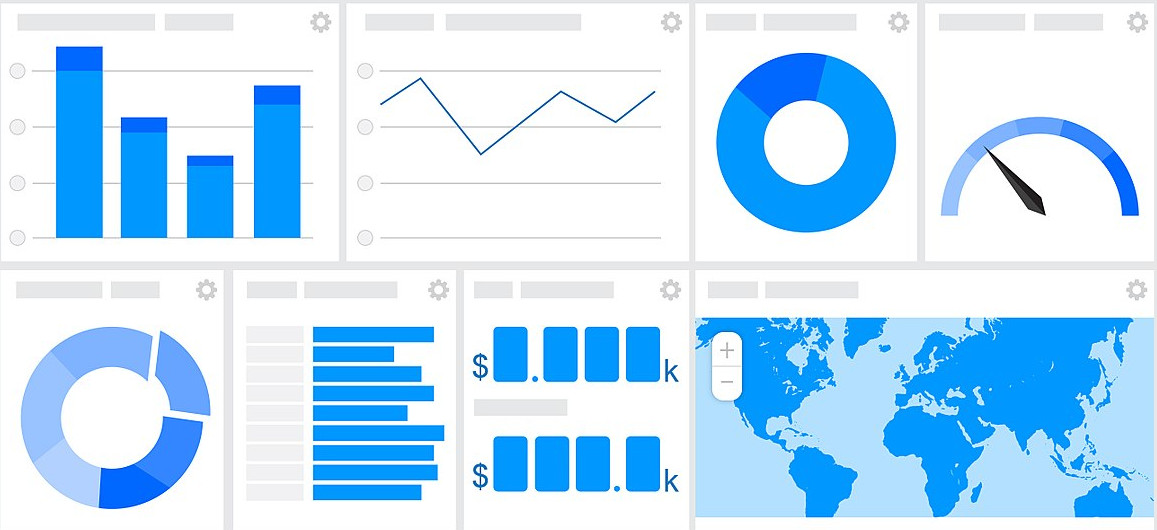
\includegraphics[width=0.5\textwidth]{../../images/dashboard.jpg}
%        %\caption{Digital Learning \label{fig:digital_learning}}
%        \\ \small \url{https://commons.wikimedia.org/}
%
%    \end{figure}
%
%    To achieve this, we utilize the built-in Moodle \underline{\textbf{Analytics API}}, 
%    which considers \underline{\textbf{Indicators}} as independent variables and the 
%    \underline{\textbf{Target}} as the dependent variable.
%
%\end{frame}
%
%\begin{frame}{Context}
%    Moodle comes with default indicators and targets, and it is possible to extend its 
%    classes to define custom indicators and targets based on Moodle data. 
%
%    \begin{figure}[H]
%        \centering
%        
\includegraphics[width=0.5\textwidth]{../../images/moodle.jpg}
%        %\caption{Digital Learning \label{fig:digital_learning}}
%        \\ \small \url{https://moodle.org}
%        % https://commons.wikimedia.org/wiki/File:Infruid%27s_Self-Service_BI_Tool_Dashboard.jpg
%        % https://fr.m.wikipedia.org/wiki/Fichier:Computer_science_education.png
%    \end{figure}
%
%    However, we aim to incorporate external data into Moodle to be used 
%    as additional indicators and targets.
%\end{frame}
%
%\subsection{Research Questions}
%\begin{frame}{Research Questions}
%    \begin{enumerate}[<+-|alert@+>]\color{gray}
%        \item What kind of external data can be usefully and safely integrated with 
%              the Moodle (behavioral) data?
%        \item How this enriched data can be used as features for statistical and 
%              Machine Learning models (to be presented in dashboards) respecting privacy and student autonomy ?
%    \end{enumerate}
%\end{frame}
%
%\begin{frame}{Introdução}
%    Um exemplo com referência
%    \cite{byron2012usingdrupal}
%\end{frame}
%
%\begin{table}[H]
%    \caption{Tertiary Review Databases}
%    \label{table:tertiary_review_database}
%    \begin{tabular}{c|c}
%    \toprule
%     & 0 \\
%    database &  \\
%    \midrule
%    acm & 64 \\
%    engineering village & 13 \\
%    ieee & 1 \\
%    science direct & 70 \\
%    scopus & 26 \\
%    web of science & 13 \\
%    \bottomrule
%    \end{tabular}
%    \end{table}
%    
%
%% timeline % qualificação
%% Advances since last pitch
%% Ongoing and Future Work Plan OR Next steps
%%Research Questions
%% The road until now
%
%
%\section{Tertiary Review}
%
%%% Contar o processo antes de decidirmos fazer a revisão terciária, e parte exploratória
%
%%% Colocar projetos/implementações de LAD que existem
%
%%% Descrever o overleaf
%
%%\textit{Learning Analytics Dashboards} ou simplesmente \textit{LAD} é um mecanismo muito recente de suporte ao processo de ensino e aprendizagem e portanto ainda conta diversas lacunas em suas possíveis potencialidades e limitações, neste sentido faz-se necessário um levantamento do estado da arte desse campo de pesquisa através da sistematização por revisão sistemática (RS).  
%%
%%\textit{LAD} ainda é uma área interdisciplinar que envolve áreas como Ciência da Computação, Ciência de Dados, Educação e Psicologia, entre outras. Devido a interdisciplinaridade em estudos com \textit{LAD}, muitos trabalhos primários ou mesmo secundários apresentam viéses que refletem o campo de estudos dos pesquisadores, além disso RS tendem a ficar defesadas rapidamente. Sendo assim vamos nesta seção realizar uma revisão terciária em \textit{LAD} e verificar a necessidade ou não de uma nova RS em \textit{LAD}, ou para atualização de RS já existente ou que fundamente uma RS com um novo enfoque não abordado até então. 
%
%Desde a última década tem surgido estudos de revisão sistemática em \textit{LAD}, nesta revisão terciária, fizemos o levantamento nas 6 bases de dados seguintes, sem restrição de data.
%
%\begin{itemize}
%    \begin{spacing}{0.5}
%      \item ACM Digital Library
%      \item Elsevier Science Direct
%      \item Engineering Village El Compendex
%      \item IEEE Xplore Digital Library
%      \item Scopus
%      \item Web of Science
%    \end{spacing}
%\end{itemize}
%
%A escolha dessas bases de dados é porque nosso interesse de pesquisa está mais próximo da área de engenharia de software, então não selecionamos bases de dados que tenham enfoque em trabalho exclusivamente de educação ou psicologia, duas áreas que contém bastante pesquisas em \textit{LAD}.
%
%\begin{figure}[H]
%  \centering
%  \includegraphics[width=0.8\textwidth]{../outputs/tertiary_review_yearly_barplot.pdf}
%  \caption{ddd}
%  \label{fg:tertiary_review_yearly_barplot}
%\end{figure}
%
%Como pode ser observado no gráfico da figura \ref{fg:tertiary_review_yearly_barplot}, nas bases consultadas, a primeira revisão sistemática encontrada com \textit{LAD} foi em 2014. Deste então esse número vem aumentando. A quantidade total de RS encontra foi 189, conforme tabela \ref{table:tertiary_review_database}, que mostra a quantidade de RS por cada base de dados.
%
%\input{../outputs/tertiary_review_database.tex}
%
%Das 189 RS encontradas, 15 foram selecionadas conformo os critérios de inclusão e exclusão definidos no protocolo da revisão terciária (ainda será inserido). Desdes 15, 6 tinham como critérios de seleção aspectos que avaliavam se os estudos primários (EP) tinham ou não fundamentos educionais na implementação do \textit{LAD}, 6 avaliaram EP de forma mais ampla, sem se prender ao critério específico, 2 tinham como critério de seleção averiguar se os EP continham métodos de validar o uso do \textit{LAD} e sua efetividade no ganho educacional, e somente 1 avaliou se os EPs utilizavam-se de mecanimos de Aprendizado de Máquina.
%
%Nenhuma RS das bases consultadas, levou em consideração \textit{LADs} implementadas para o LMS mais popular do mundo, o moodle, e de forma mais ampla, nenhuma RS considerou \textit{LAD} implementado em código aberto, assim, neste trabalho propomos uma RS de \textit{LAD} : 1) implementadas como plugin do Moodle e 2) \textit{LAD} que não foram implementadas no Moodle, mas foram desenvolvidas e licenciada como códido aberto. Acreditamos que \textit{LAD}, sendo uma área em constante crescimento, a implementação em código aberto, pode trazer o benefício de aumentar a comunidade envolvida nessa área de pesquisa, deixando mais opções disponiveis a comunidade que trabalha com \textit{LAD}.
%
%
%\subsection{Dificuldades na Tertiary Review}
%
%A principal dificuldade referente a realização da TR foi na exportação das referências no formato bibtex, pois duas bases de dados não exportaram arquivos bibtex bem formatados. A base Engineering Village na mesma referência utilizou a chave copyright multiplas vezes. Já a base Scopus não usou idenficador único para cada artigo. Em ambos casos o arquivo bibtex foi corrigido manualemte. 
%
%\cite{ferreira2012}
%


